\documentclass[11pt]{scrartcl}
\usepackage{amsmath}
\usepackage[sexy,mdthm,secthm]{evan}
\usepackage[margins=1.0in]{geometry}
\usepackage{amssymb}
\usepackage[utf8]{inputenc}

\newcommand{\p}[2]{\frac{\partial {#1}}{\partial {#2}}}
\newcommand{\inv}[1]{\frac{1}{#1}}
\newcommand{\fl}[1]{\lfloor #1\rfloor}
\newcommand{\cl}[1]{\lceil #1\rceil}

%fix margins
\usepackage[letterpaper,top=2cm,bottom=2cm,left=3cm,right=3cm,marginparwidth=1.75cm]{geometry}
%\setcounter{section}{-1}

\setlength{\parskip}{\baselineskip}%
\setlength{\parindent}{0pt}%
\usepackage{mathtools}
\usepackage{amssymb}
\usepackage{amsfonts}
% \usepackage{asymptote}
\newcommand*\conj[1]{\bar{#1}}
\newcommand{\ord}{\text{ord}}
\newcommand{\T}{\textbf{T}}
\newcommand{\H}{\textbf{H}}
\documentclass{article}
\usepackage[utf8]{inputenc}
\usepackage[dvipsnames]{xcolor} % let LaTeX work with colors
\usepackage{framed} % useful for creating "boxes"

%seperate sections in seperate pages
% \usepackage{titlesec}
% \newcommand{\sectionbreak}{\clearpage}

\colorlet{shadecolor}{orange!15} % I like orange-colored boxes.

\usepackage{amsthm}
\title{EGMO Chapter 8: Inversion}
\author{Ryan Yang}
\date{May 2021}

\begin{document}

\maketitle

\section{Problem 8.25}
\begin{problem}
Let $A,B,C$ be three collinear points and $P$ be a point not on this line. Prove that the circumcenters of $\triangle PAB, \triangle PBC,$ and $\triangle PCA$ lie on a circle passing through $P$. 
\end{problem}
\begin{soln}
Let $X,Y,Z$ be the centers of $\triangle PAB, \triangle PBC,$ and $\triangle PCA$.  We invert around $P$ with radius 1. 

Thus, due to lemma 8.10, we have that $X'$ is the reflection of $P$ over $A'B'$.

However, as a property of inversion we will have that $ABC\to A'B'C'$ where $A'B'C'$ is a circle which passes through $P$. Thus, by Simson's the feet from $P$ to each side are collinear, and a homothety of factor $\times 2$ gives us that $X',Y',Z'$ are collinear.

Inverting back, this clearly gives us that $P\in (XYZ)$ and we are done.
\end{soln}

\section{Problem 8.26 - BAMO 2008/6}
% 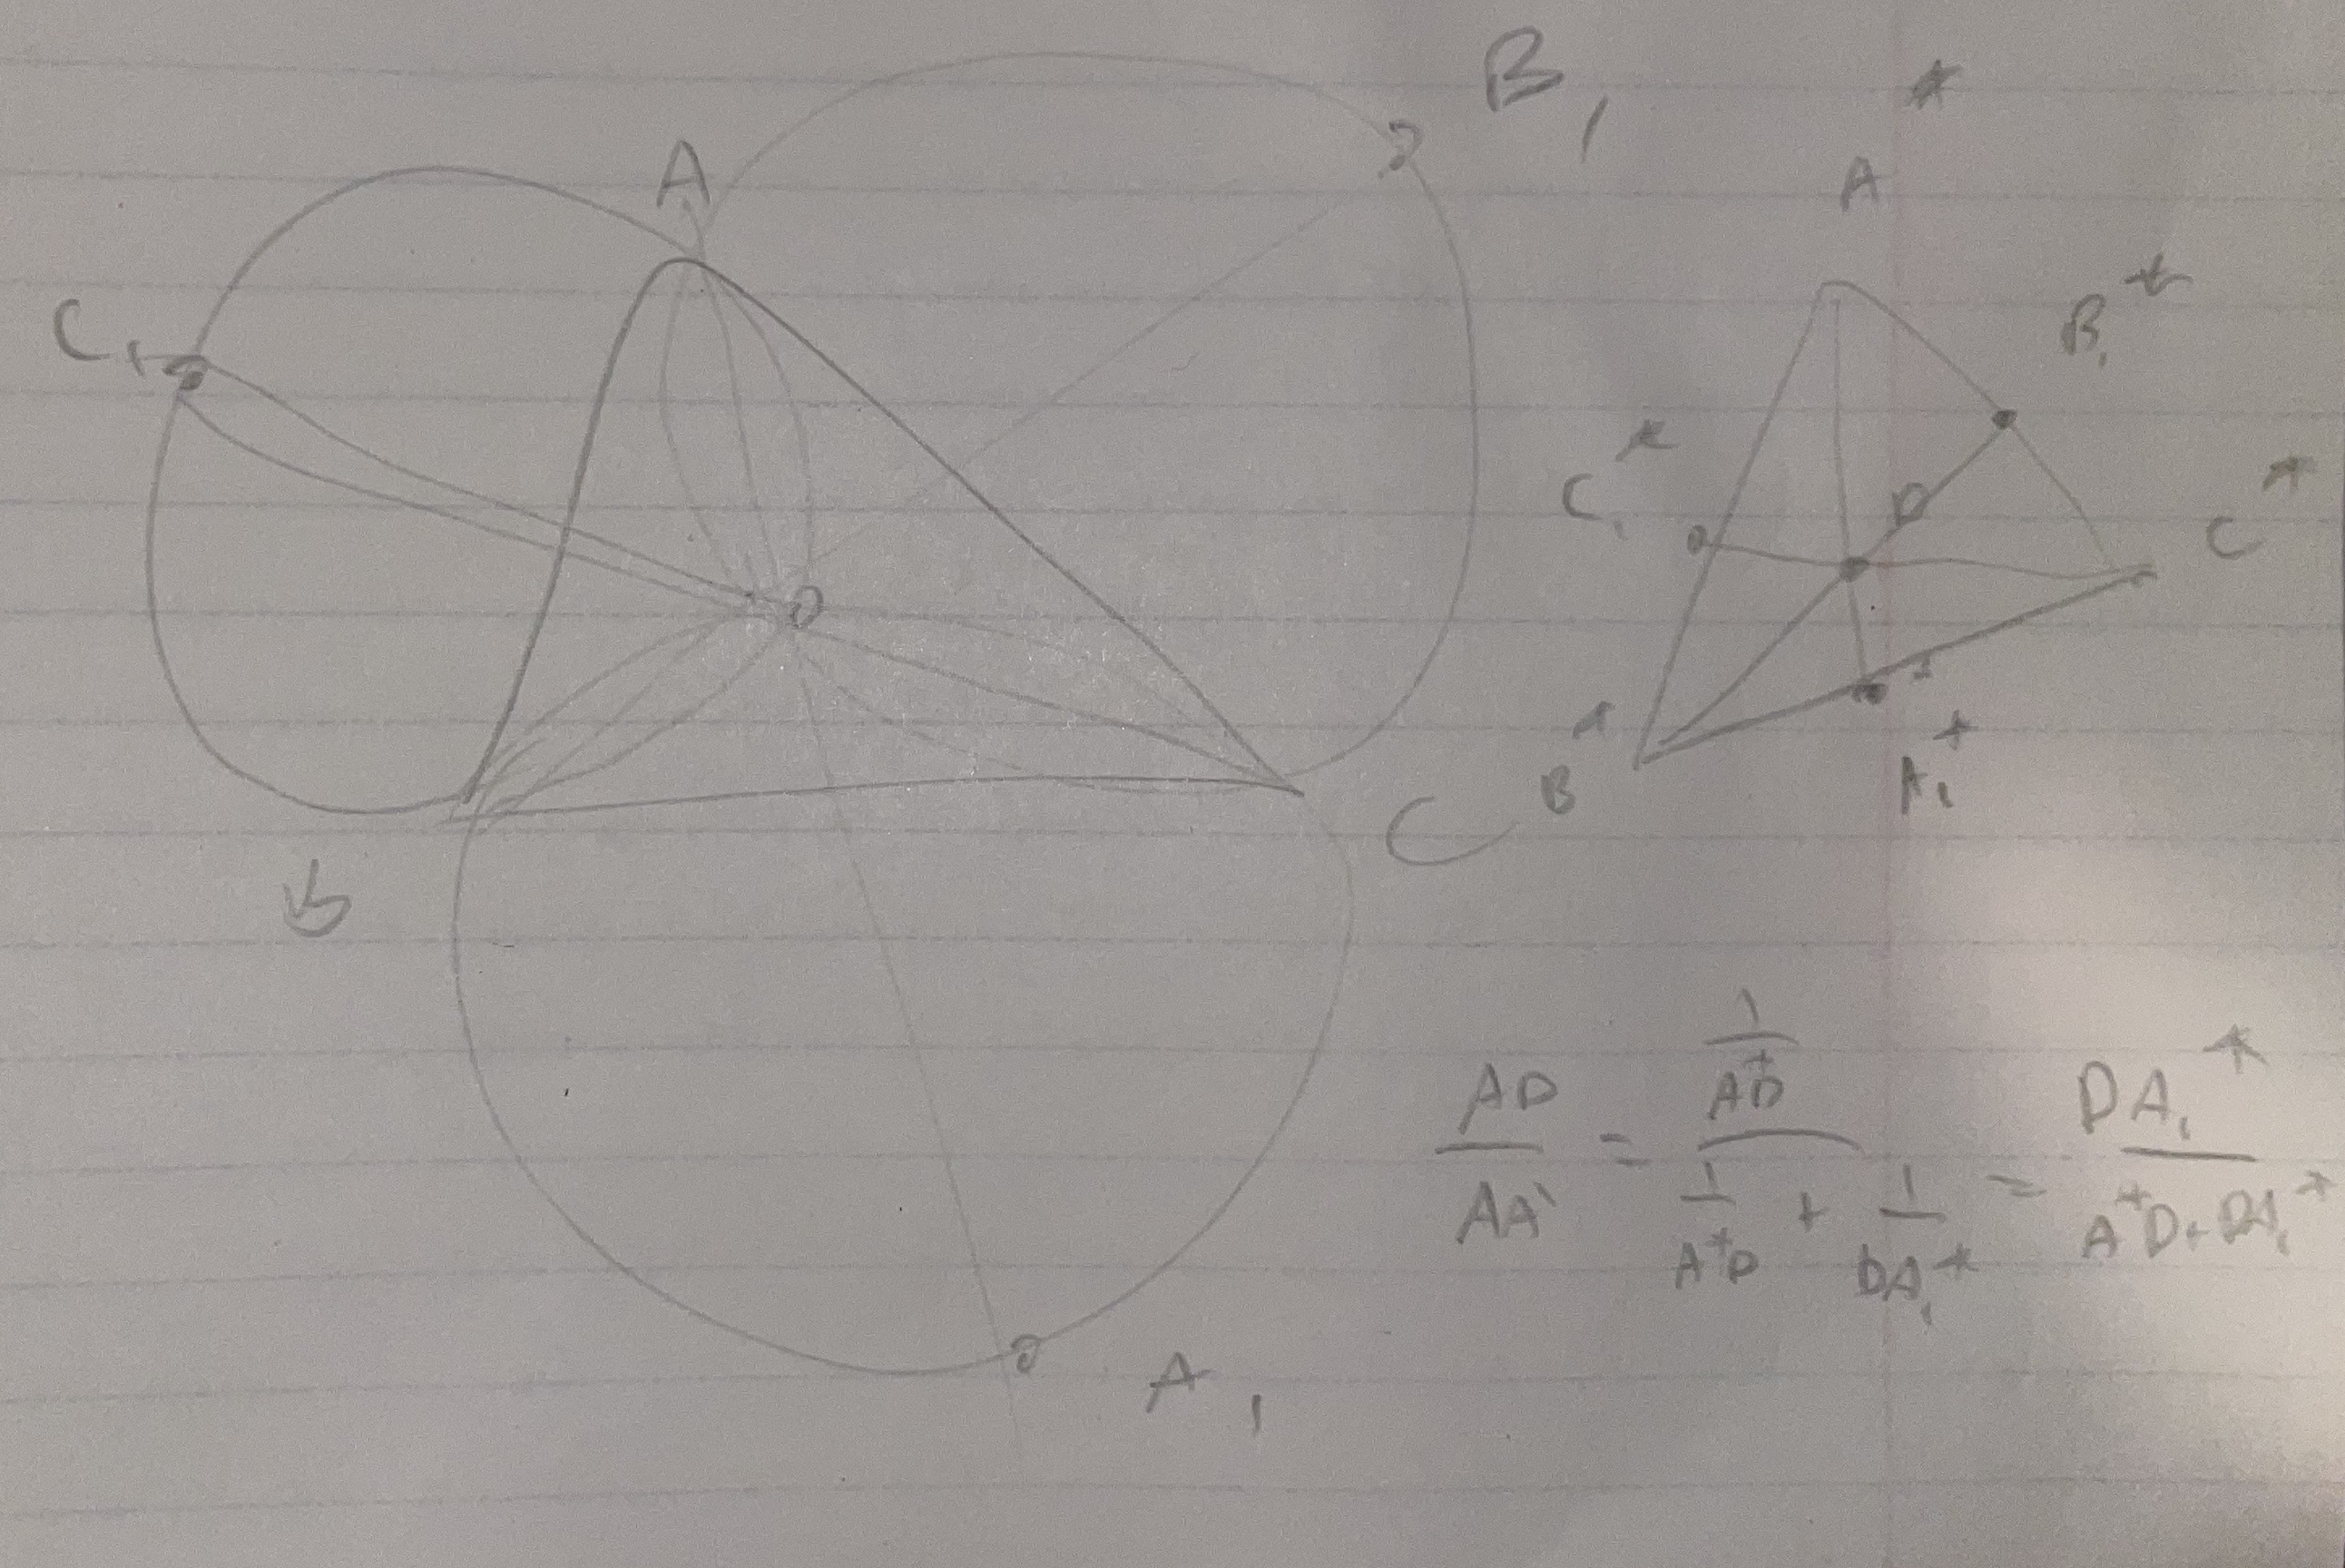
\includegraphics[scale=0.3]{26.png}

Invert about $D$ with a circle of radius 1. Note that $(BDCA_1)$ cyclic implies $B'A_1'C'$ are all collinear. Similar results by symmetry on other sides.

Then, 
\[\frac{AD}{AA_1} = \frac{AD}{AD+DA_1}=\frac{\frac{1}{AD'}}{\frac{1}{AD'}+\frac{1}{DA_1'}}=\frac{DA_1'}{DA_1'+A'D} = \frac{DA_1'}{AA_1'}\]
Thus sum of this becomes, with second equality due to Area ratio's.
\[\frac{AD}{AA_1}+\frac{BD}{BB_1}+\frac{CD}{CC_1} = \frac{DA_1'}{AA_1'}+\frac{DB_1'}{BB_1'}+\frac{DC_1'}{CC_1'} = \frac{[B'D'C']+[C'DA']+[A'DB']}{[A'B'C']}=1\]
and we are done $\blacksquare$.

\section{Problem 8.27 - Iran Olympiad 1996}
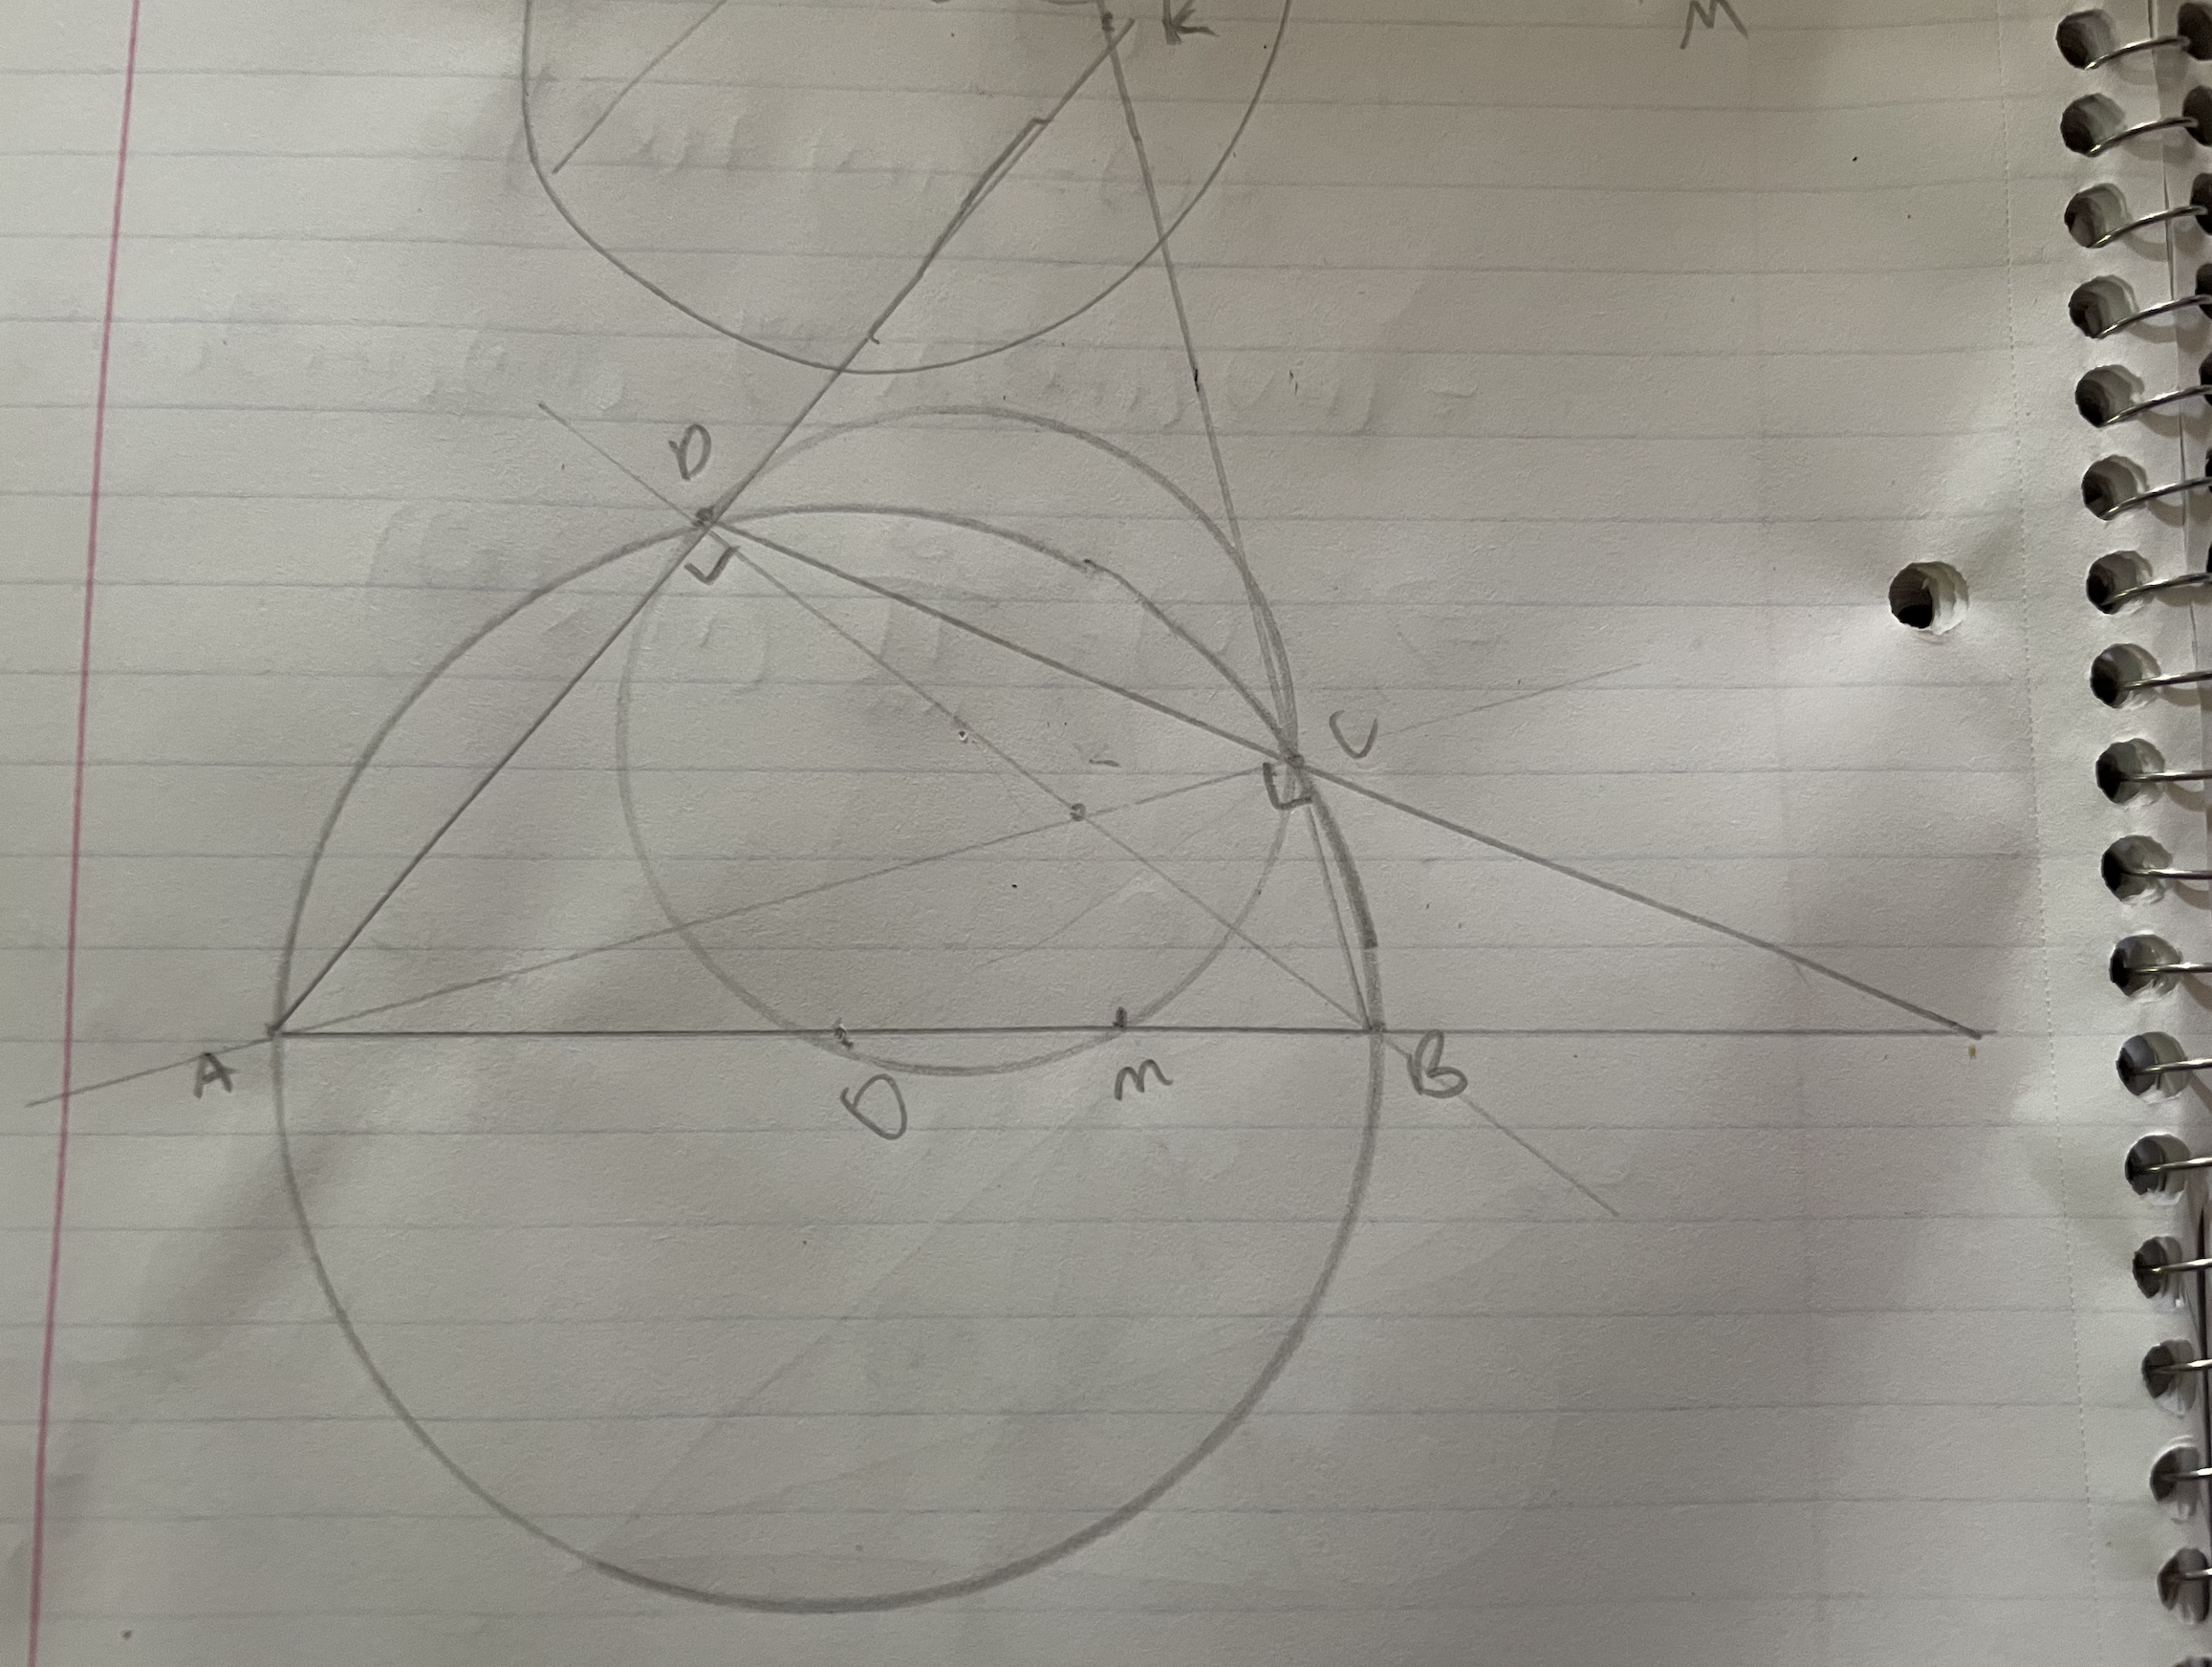
\includegraphics[scale=0.3]{27.png}

Invert about $\omega$, the semicircle. Note that $A,B,C,D$ were free in the original diagram, and will be sent to themselves post inversion. Next, since $M=AB\cap CD$, we have that $M^* = AB\cap (COD)$. 

Next, $K=(AOC)\cap (BOD)$, since (AOC) passes through the center of inversion, it will get sent to a line through $AC$. Similarly $(BOD)\to \overline{BD}$. Thus, we have $K^* = AD\cap BC$.

Now, simply note that (COD) is the 9-point circle of $\triangle KAB$, thus $M$ must be the foot of the altitude from $K$ so we have $\angle KMO=90$ and we are done $\blacksquare$.

\section{Problem 8.28 - Shortlist 2003/G4}
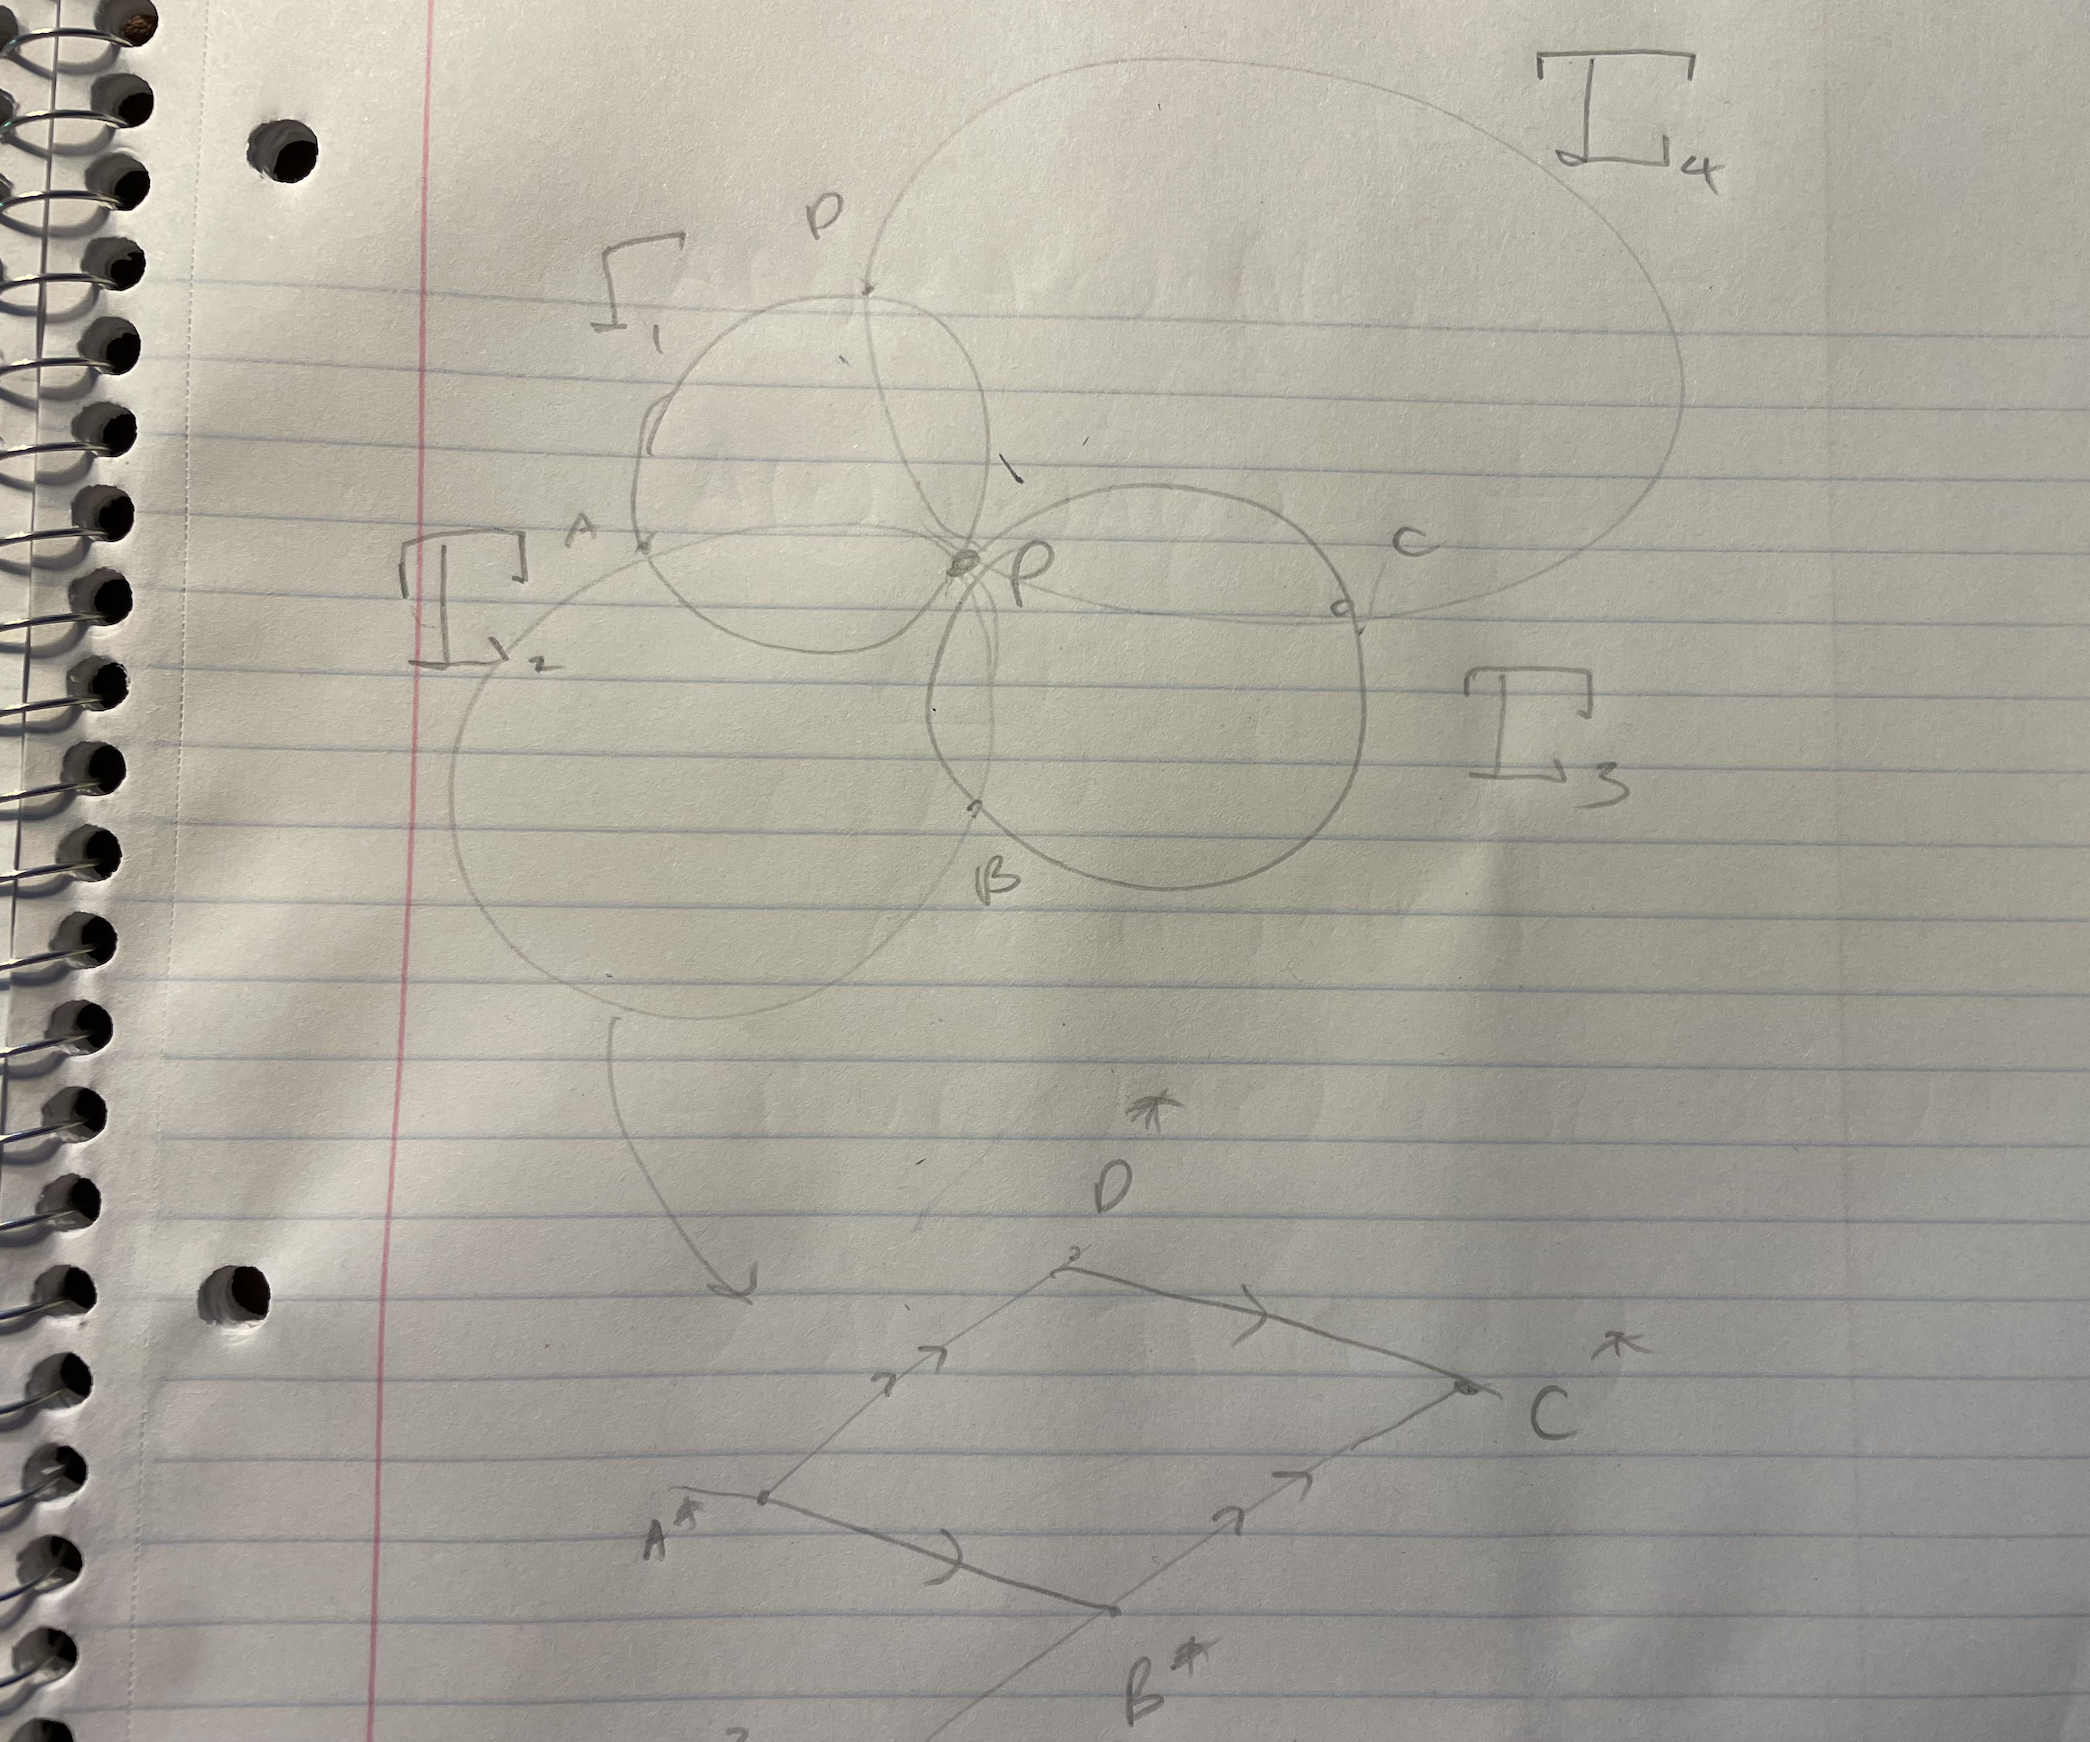
\includegraphics[scale=0.3]{28.png}\\
We rename $P$ to $O$. Invert about $O$ with radius 1. Note that since $\Gamma_1$ is tangent to $\Gamma_3$, we will have $A^*D^*\parallel B^* C^*$, and similarly $\Gamma_2$ tangent to $\Gamma_4$ implies that $A^*B^*\parallel C^* D^*$.

Thus, $A^*B^*C^*D^*$ is a parallelogram, so $A^*B^*=C^*D^*$ and $A^*D^*=B^*C^*$.

Now, we evaluate using Inversion Distance Formula,
\[\frac{AB\cdot BC}{AD\cdot DC} = \frac{\frac{A^*B^*}{OA^*OB^*}\cdot \frac{B^*C^*}{OB^*OC^*}}{\frac{AD^*}{OA^*OD^*}\cdot \frac{D^*C^*}{OD^*OC^*}} = \frac{{OD^*}^2}{{OB^*}^2}\cdot \frac{A^*B^*\cdot B^*C^* \cdot OA^*\cdot OC^* }{C^*D^*\cdot A^*B^*\cdot OA^*\cdot OC^*} = \frac{{OD^*}^2}{{OB^*}^2}= \frac{OB^2}{OD^2}\]
and we are done $\blacksquare$.

\section{Problem 8.29 - $IO$ passes through the centroid of the contact triangle}
Note that due to Lemma 8.11, the inversion with respect to the incircle sends $\Gamma$, the circumcircle,  to the nine-point circle of $\triangle DEF$.  Let the nine-point circle have center $N_9$.

Now, by proposition $8.6$, we have that the centers of the two circles are collinear with the center of inversion, so $I,O,N_9$ are collinear.

However, the Euler Line of $\triangle DEF$ is $I$(circumcenter), $G_1$(median) and $N$(nine-point center of $\triangle DEF$. Thus, combining $ION$ and $IG_1N$, we have $IOG_1$ collinear and we are done.


\end{document}
